\def\QRCODE{TB_image_TUT.IMG.image_enhancement_matlabqrcode.png}
\def\QRPAGE{http://www.iptutorials.science/tree/master/TB_image/TUT.IMG.image_enhancement/matlab}
\mcorrectionsection{Matlab correction}

\subsection{Intensity transformations}
At first, the image is normalized between 0 and 1.
\begin{matlab}
A=imread('osteoblaste.tif');
A=double(A);
A=A/255; % ensure values between 0 and 1
\end{matlab}

\subsubsection{Gamma transform}
The \matlabregistered{} function \minline{imadjust} is used to adjust gamma. Be careful that the range given in argument does not imply a strict gamma correction. Results are shown in Fig.\ref{fig:enhancement:matlab:gamma}.
\begin{matlab}
figure
subplot(2,2,1);imshow(A);title('original image');

Ar=imadjust(A,[min(min(A)) max(max(A))],[0 1],1);
subplot(2,2,2);imshow(Ar);title('enhanced, g=1');

Ar=imadjust(A,[0.25 0.75],[0 1],0.5);
subplot(2,2,3);imshow(Ar);title('enhanced, g=0.5');

Ar=imadjust(A,[0.25 0.5],[0 1],2);
subplot(2,2,4);imshow(Ar);title('enhanced, g=2');
\end{matlab}

\begin{figure}[htbp]
 \centering
 \subfloat[Original image.]{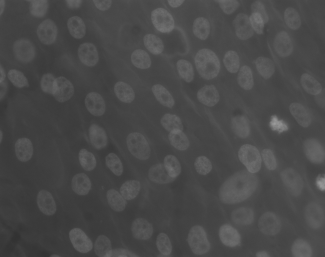
\includegraphics[width=.4\linewidth]{osteoblaste.png}}
 \hfill
 \subfloat[$\gamma=1$.]{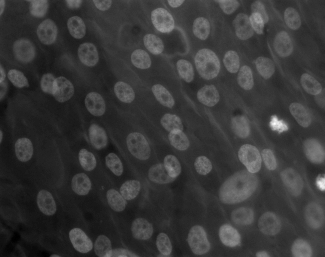
\includegraphics[width=.4\linewidth]{osteo_g1.png}}
 
 \subfloat[$\gamma=2$.]{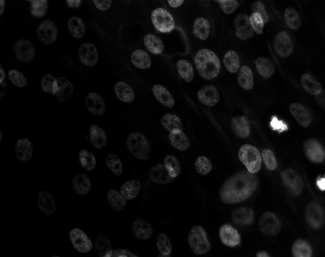
\includegraphics[width=.4\linewidth]{osteo_g2.png}} \hfill
 \subfloat[$\gamma=0.5$.]{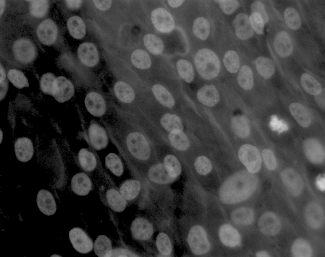
\includegraphics[width=.4\linewidth]{osteo_g05.png}}
 
 \caption{Gamma transform. Notice that these transforms are not exactly gamma transforms (due to the range in argument).}
 \label{fig:enhancement:matlab:gamma}
\end{figure}

\subsubsection{Contrast stretching}
The function used will tend to saturate values, see Fig.\ref{fig:enhancement:matlab:stretching}. 
\begin{matlab}
m=mean(mean(A));
figure
subplot(2,2,1);imshow(A);title('original image');
Ar=1./(1+(m./(A+eps)).^5);
subplot(2,2,2);imshow(Ar);title('contrast stretching : E=5');
Ar=1./(1+(m./(A+eps)).^10);
subplot(2,2,3);imshow(Ar);title('contrast stretching : E=10');
Ar=1./(1+(m./(A+eps)).^1000);
subplot(2,2,4);imshow(Ar);title('contrast stretching : E=1000');
\end{matlab}

\begin{figure}[htbp]
 \centering
 \subfloat[Original image.]{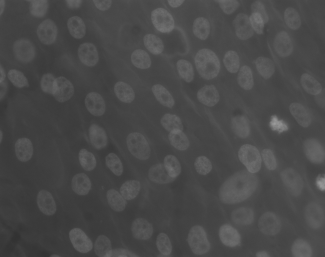
\includegraphics[width=.4\linewidth]{osteoblaste.png}} \hfill
 \subfloat[$E=5$.]{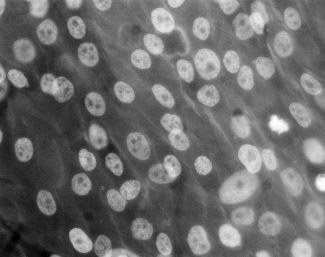
\includegraphics[width=.4\linewidth]{osteo_E5.png}}
 
 \subfloat[$E=10$.]{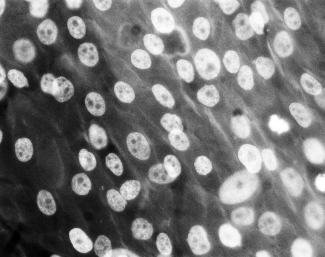
\includegraphics[width=.4\linewidth]{osteo_E10.png}} \hfill
 \subfloat[$E=1000$.]{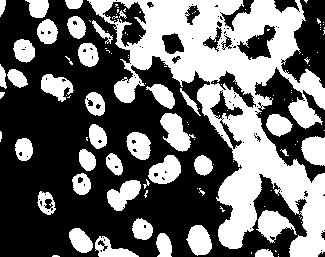
\includegraphics[width=.4\linewidth]{osteo_E1000.png}}
 
 \caption{Constrast stretching.}
 \label{fig:enhancement:matlab:stretching}
\end{figure}

\subsection{Histogram equalization}
The principle of this operation is to evaluate a lookup-table in order to perform the transformation. This LUT is the cumulative distribution function, and can be applied by using an interpolation function \minline{interp1} or the LUT function \minline{intlut}. The results are shown in Fig.\ref{fig:enhancement:matlab:histeq}.
\begin{matlab}
A=imread('osteoblaste.tif');
Ar=histeq(A);
figure
subplot(3,2,1);imshow(A);title('original image');
subplot(3,2,2);imshow(Ar);title('histogram equalization');
subplot(3,2,3);imhist(A);title('original histogram');
subplot(3,2,4);imhist(Ar);title('equalized histogram');
hnorm = imhist(A)./numel(A);
cdf=255.*cumsum(hnorm);
subplot(3,2,5);plot(1:1:256,cdf);title('LUT (cdf)');
axis([0 255 0 255]);
\end{matlab}

The previous code uses the \matlabregistered{} function for histogram equalization. You can code it as follows:
\begin{matlab}
function I2 = histo_eq(I)
%
%    histogram equalization, version with look-up-table
%    I: original image, with values in 8 bits integer
%
[hist, edges] = histcounts(I, 0:256);
cdf = cumsum(hist);
cdf = cdf / cdf(end);

% the LUT could be applied by this function:
%I2 = intlut(I, uint8(255*cdf));

I2 = interp1(edges(1:end-1), cdf, double(I(:)));
I2 = uint8(255 * I2);
I2 = reshape(I2, size(I));
\end{matlab}


\begin{figure}[htbp]
 \centering
 \subfloat[Original image.]{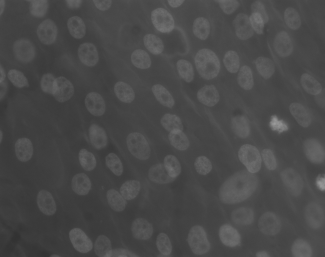
\includegraphics[width=.4\linewidth]{osteoblaste.png}}\hfill
 \subfloat[Histogram equa\-li\-za\-tion.]{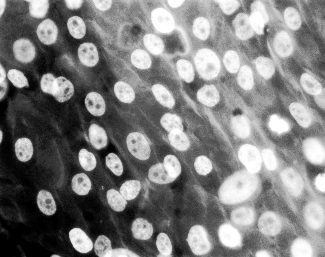
\includegraphics[width=.4\linewidth]{osteo_histeq.png}}
 
 \subfloat[Histogram of ori\-gi\-nal ima\-ge.]{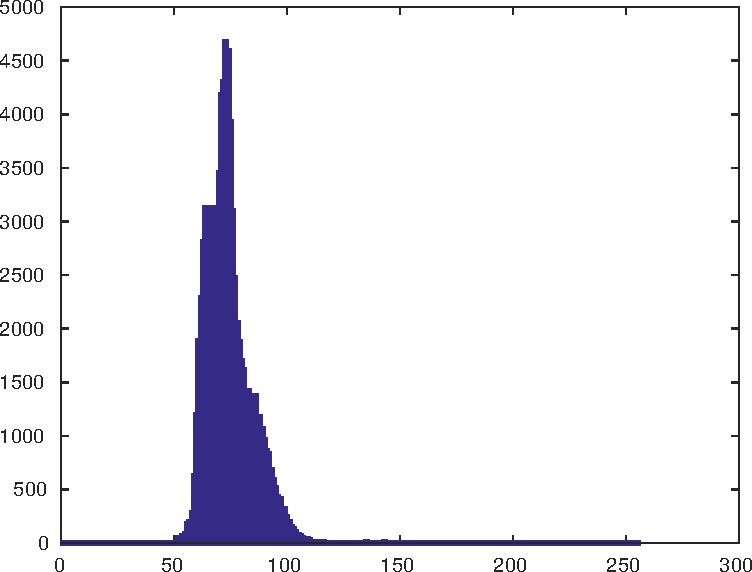
\includegraphics[width=.4\linewidth]{osteo_histogram.pdf}}\hfill
 \subfloat[Histogram of enhan\-ced image.]{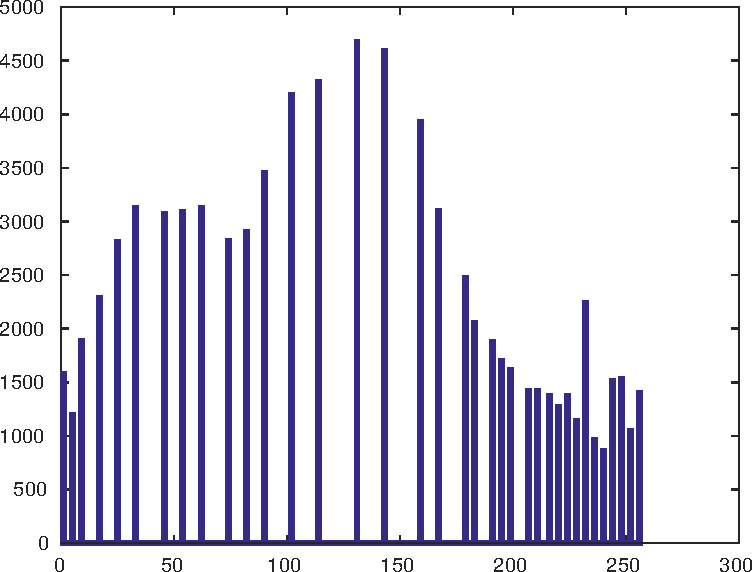
\includegraphics[width=.4\linewidth]{osteo_histogram_histeq.pdf}}

 \subfloat[LUT (cumulative distribution function).]{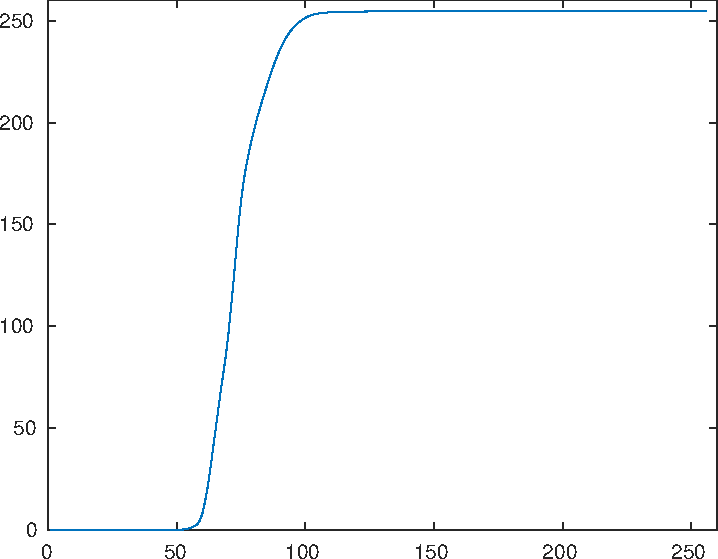
\includegraphics[width=.4\linewidth]{LUT.pdf}}
 
 \caption{Histogram equalization.}
 \label{fig:enhancement:matlab:histeq}
\end{figure}

\subsection{Histogram matching}
The histogram matching will be applied in the Phobos image (see credits).
\begin{matlab}
A=imread('phobos.jpg');
\end{matlab}

First, the function to generate the probability density function is an addition of two Gaussian functions (normalized):
\begin{matlab}
function p =twomodegauss(m1, sig1, m2, sig2, A1, A2,k)
c1 = A1*(1/((2*pi)^.5*sig1));
k1 =2*(sig1^2);
c2 = A2*(1/((2*pi)^.5*sig2));
k2 = 2*(sig2^2);
z = linspace(0,1,256);
p = k+c1*exp(-((z-m1).^ 2)./ k1)+ c2 *exp(-((z-m2).^2)./k2);
p = p./ sum(p(:));
\end{matlab}

Then, the histogram matching is performed as follows:
\begin{matlab}
% histogram to match
p=twomodegauss(0.05,0.1,0.8,0.2,0.04,0.01,0.002);

% histogram matching, \matlabregistered{} version
Ar=uint8(histeq(A,p));
figure
subplot(3,2,6);plot(p);title('model of bi-modal histogram');
xlim([0 255])
subplot(3,2,1);viewImage(A);title('original image');
subplot(3,2,2);viewImage(Ar);title('enhanced image');
subplot(3,2,3);imhist(A,256);title('original histogram');
subplot(3,2,4);imhist(Ar,256);title('matched histogram');
\end{matlab}

The \minline{histeq} \matlabregistered{} function handles histogram matching. The following code is also proposed. These are illustrated in Fig.\ref{fig:enhancement:matlab:histmatch}.

\begin{matlab}
function I2 = histo_matching(I, cdf_target)
%
%    histogram matching, version with look-up-table
%    I: original image, with values in 8 bits integer
%
[hist, edges] = histcounts(I, 0:256);
cdf = cumsum(hist);
cdf = cdf / cdf(end);

% 1st apply histogram equalization
LUT = interp1(edges(1:end-1), cdf, double(I(:)));

% the apply inverse transformation to match target cdf
im2 = interp1(cdf_target, edges(1:end-1), LUT);

% finally, reshape and convert to uint8
I2 = reshape(im2, size(I,1), size(I,2));
I2 = uint8(I2);
\end{matlab}

\begin{figure}[htbp]
 \centering
 \subfloat[Original image.]{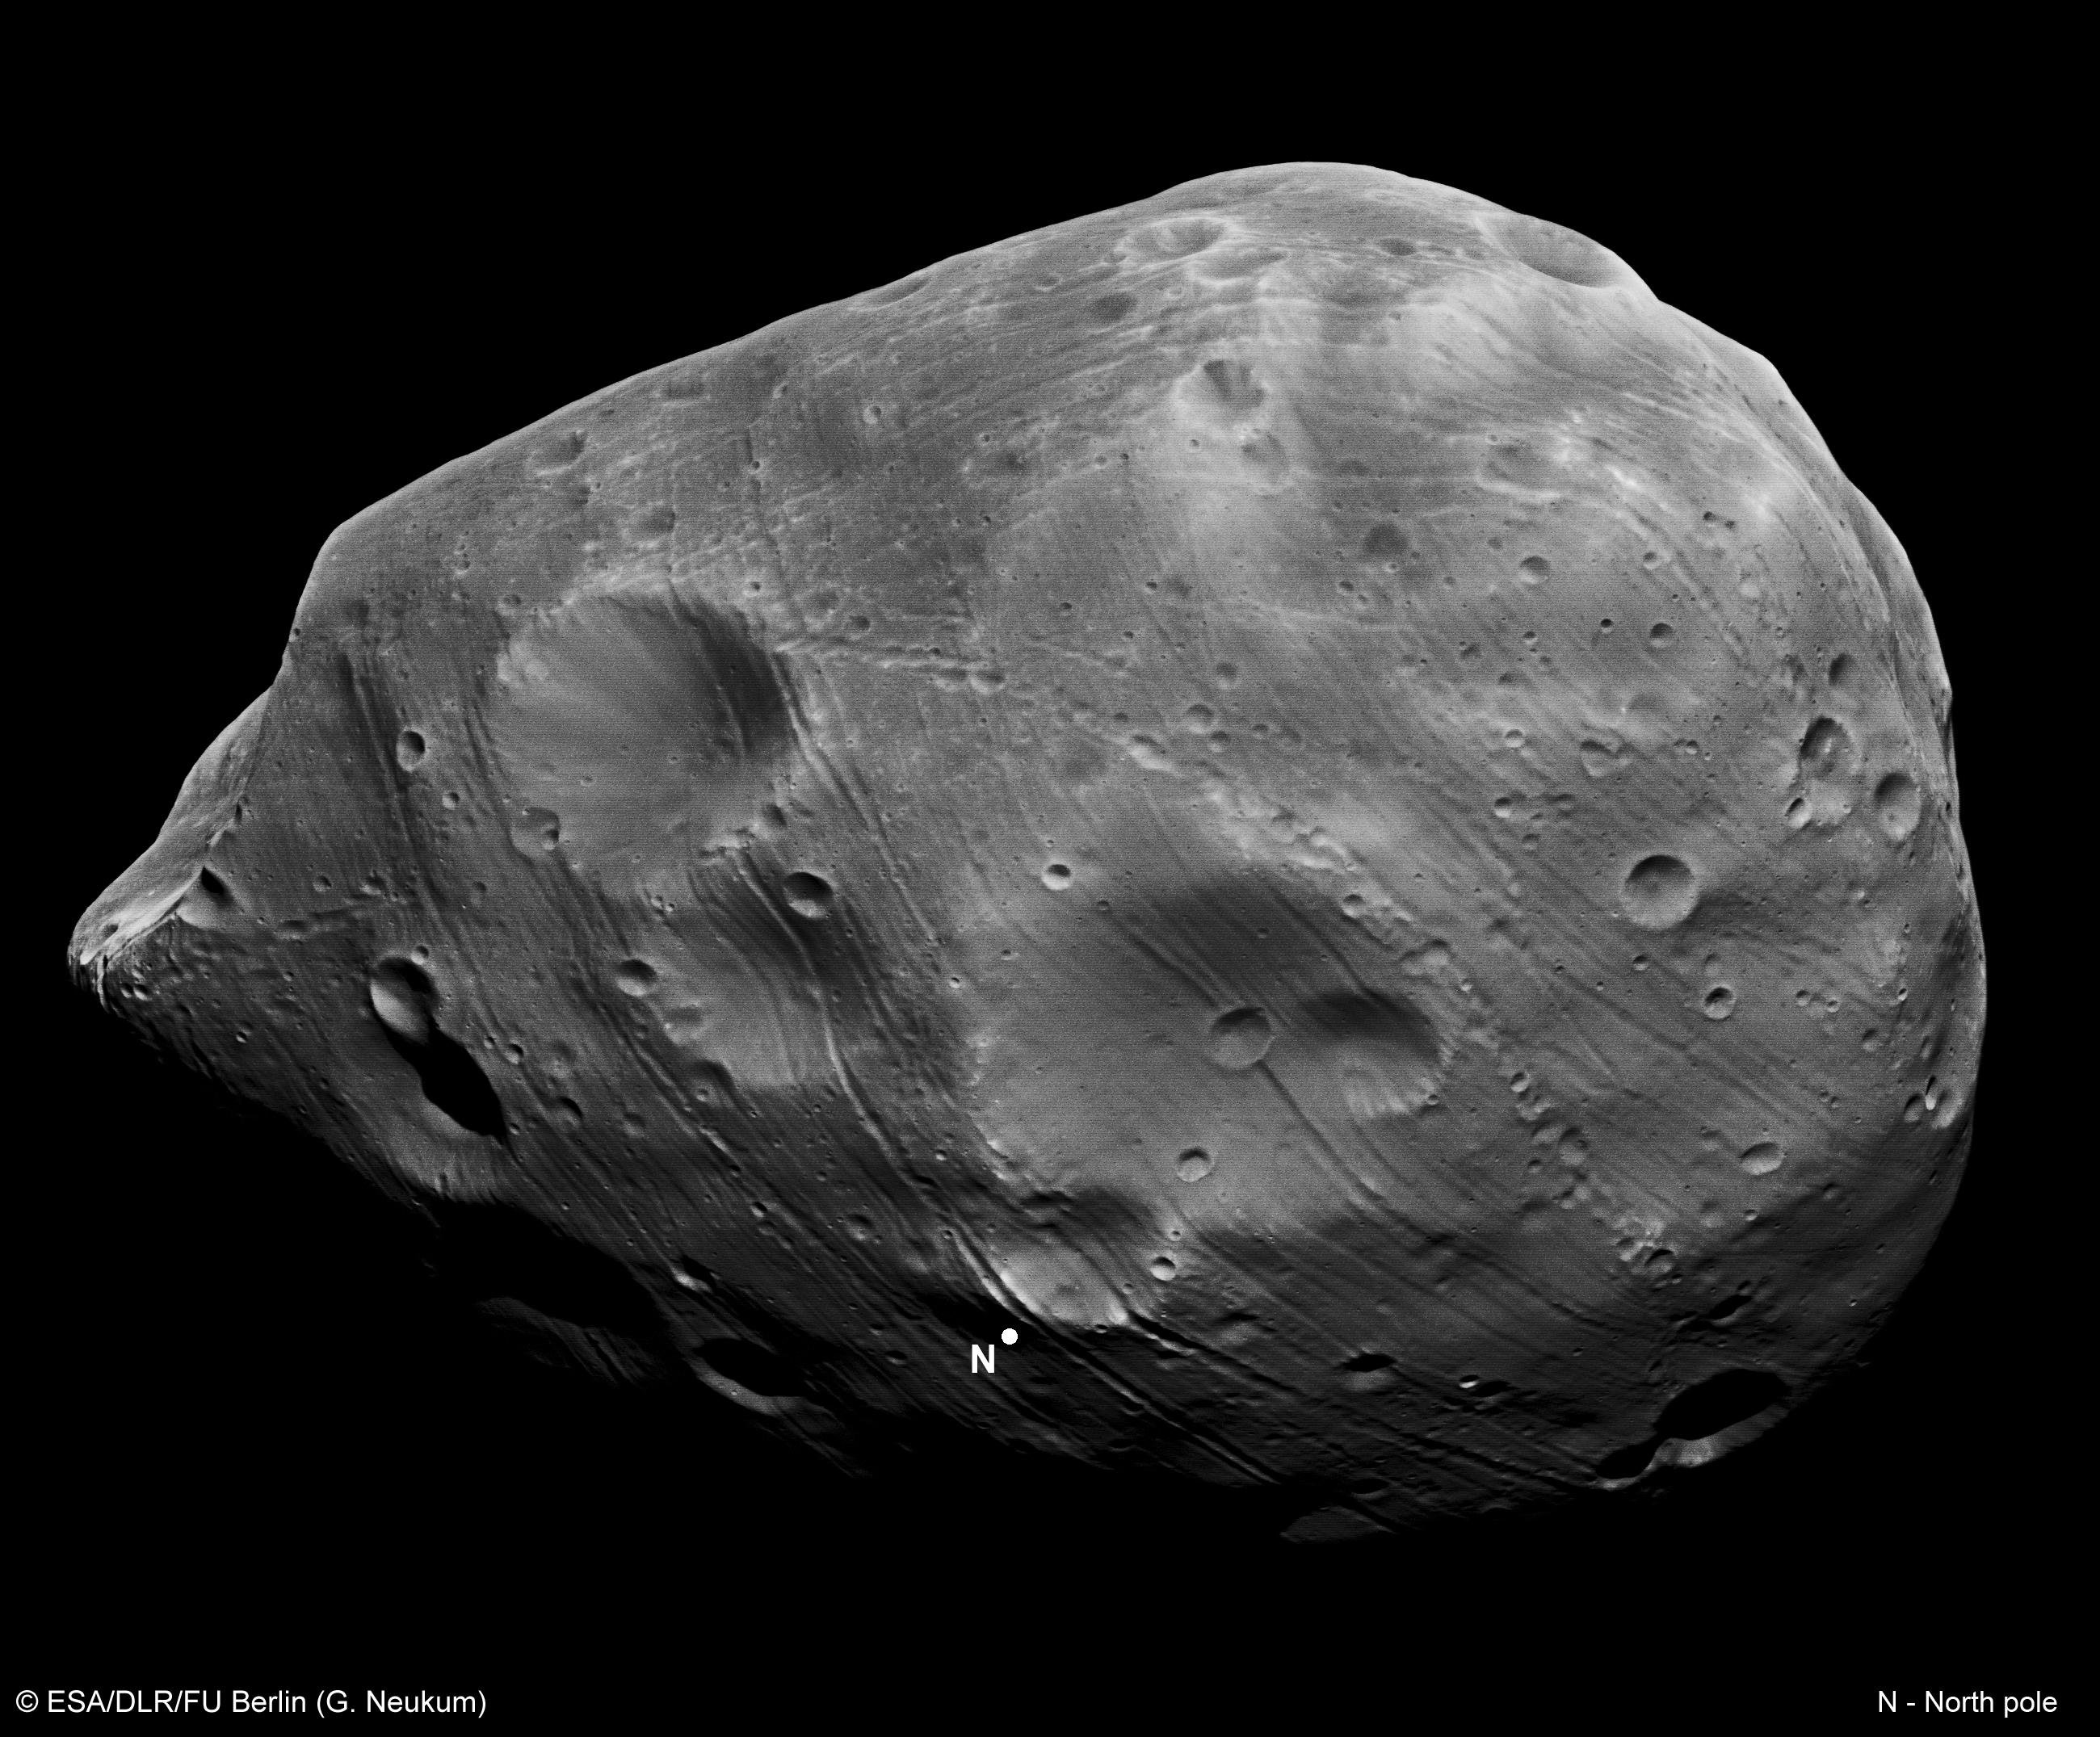
\includegraphics[width=.3\linewidth]{phobos.jpg}}\hfill
 \subfloat[Histogram equali\-za\-tion.]{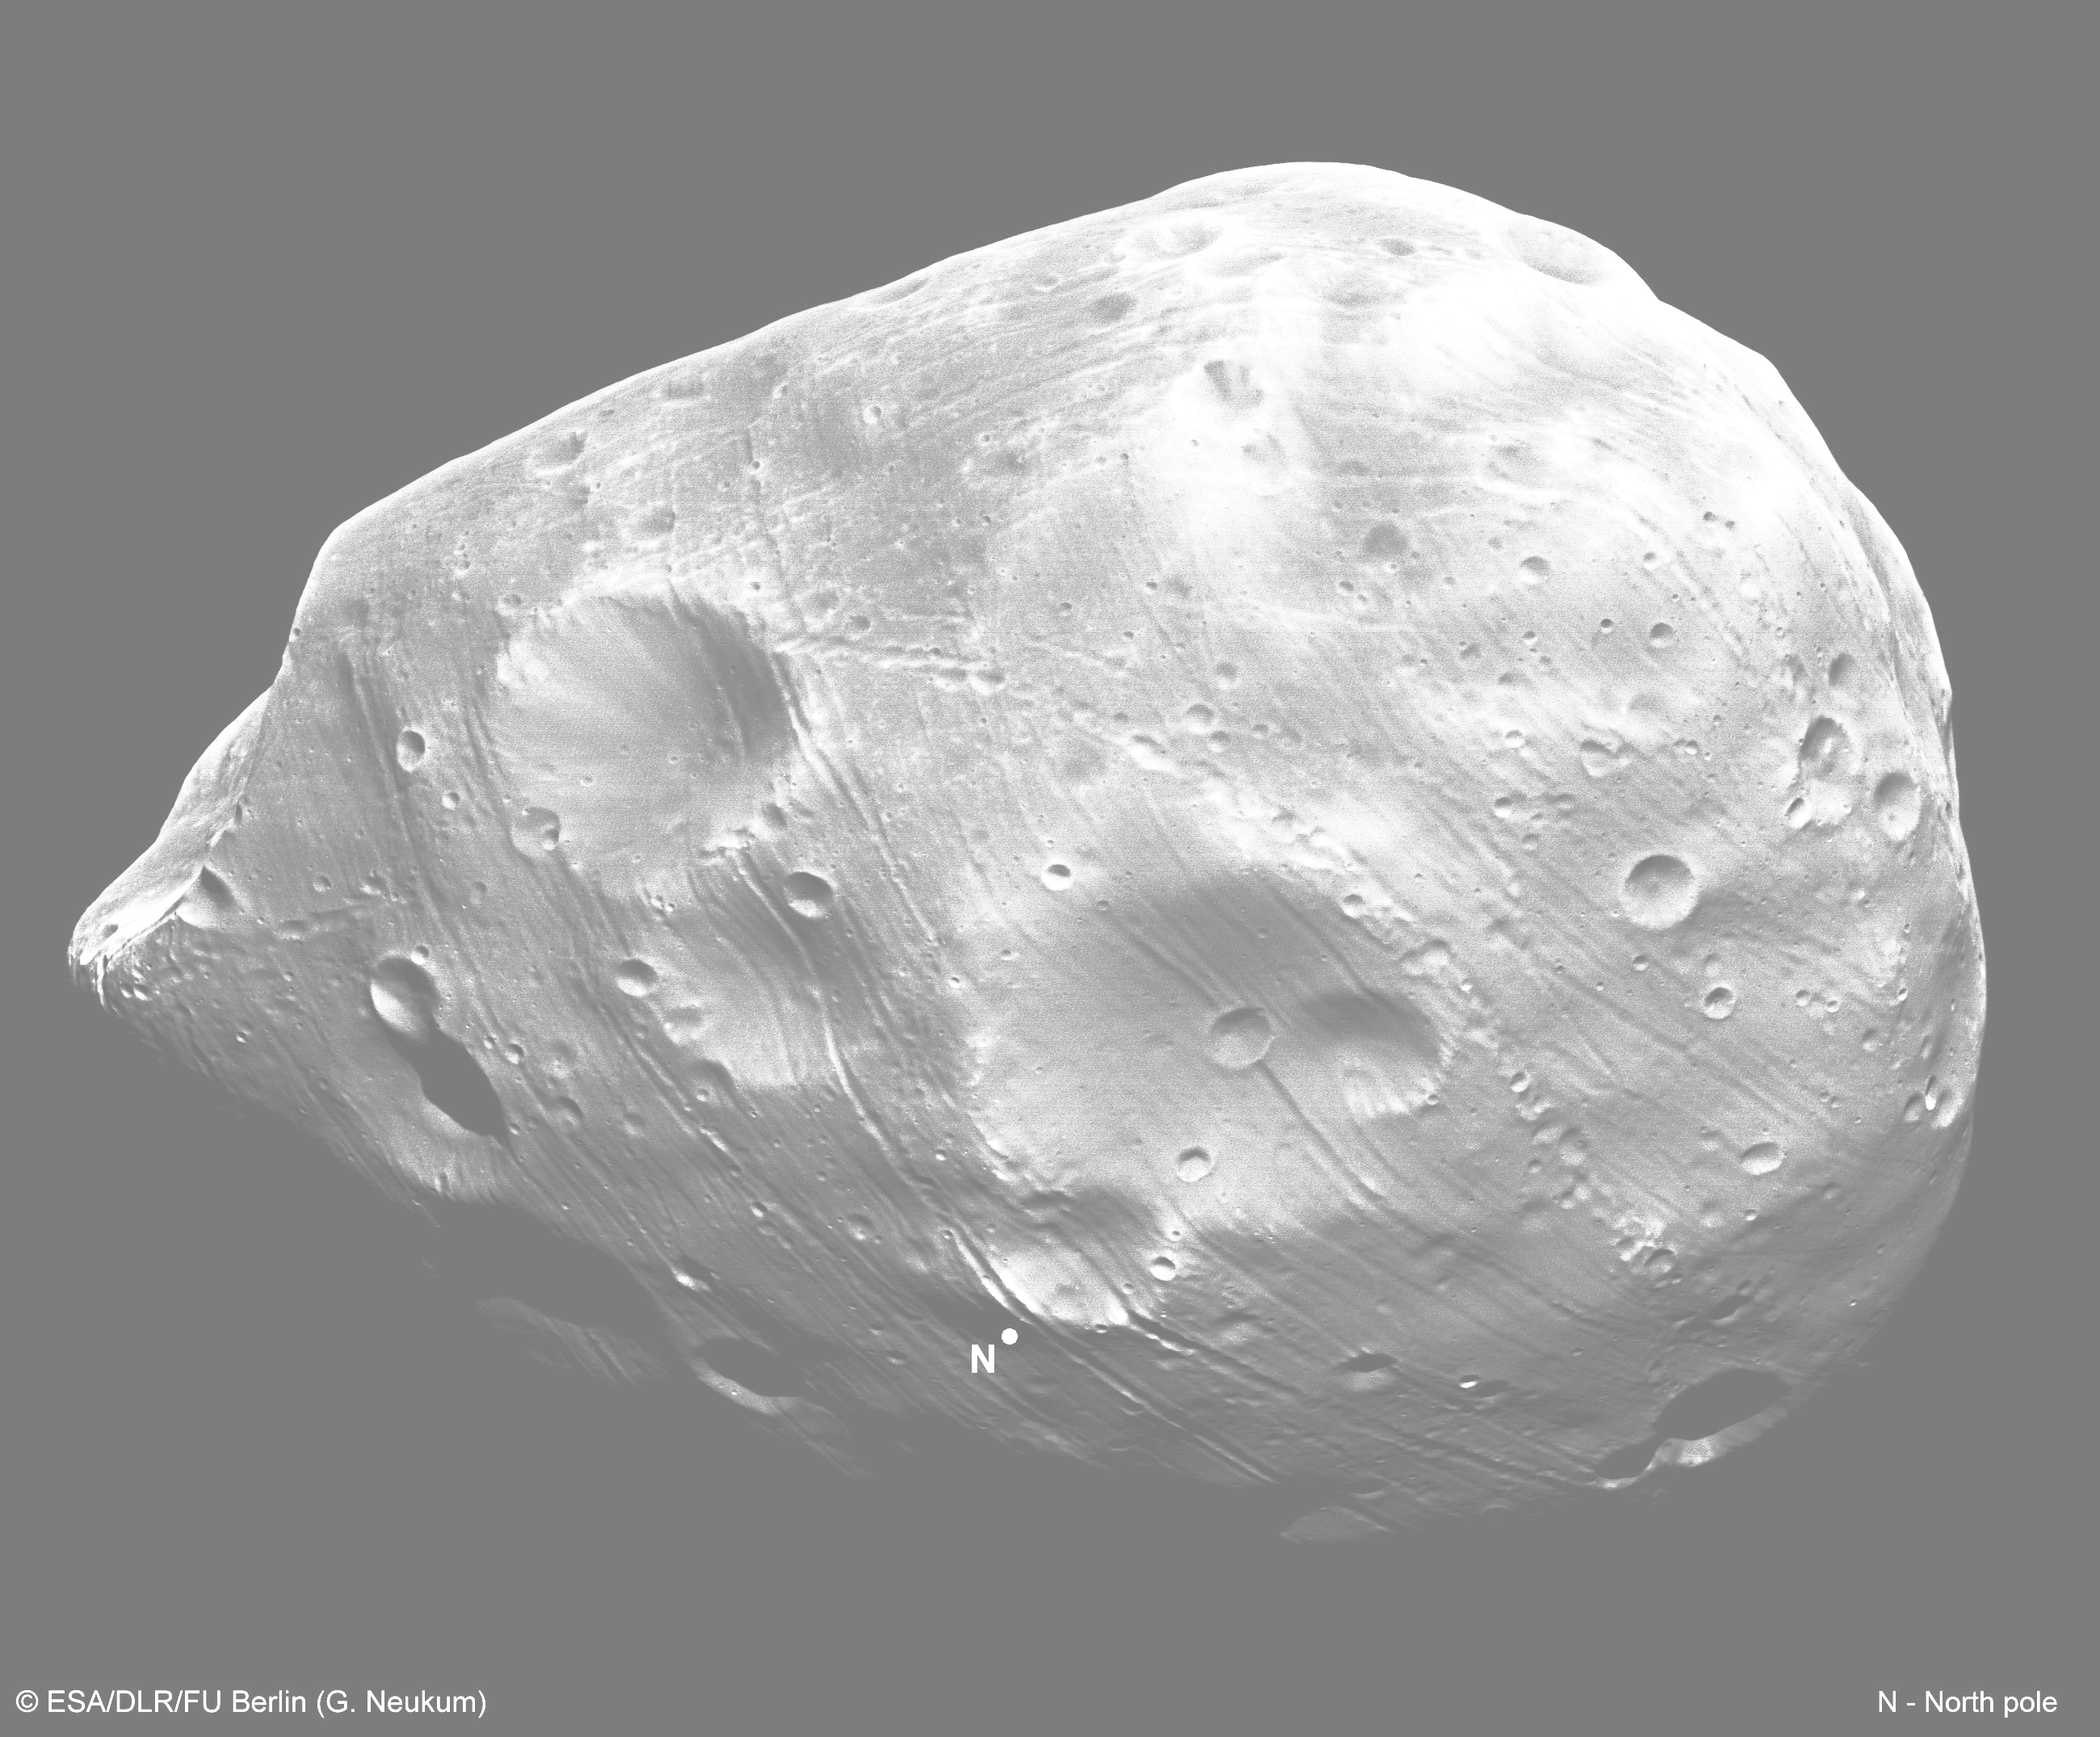
\includegraphics[width=.3\linewidth]{phobos_histeq.png}}\hfill
 \subfloat[Histogram matching.]{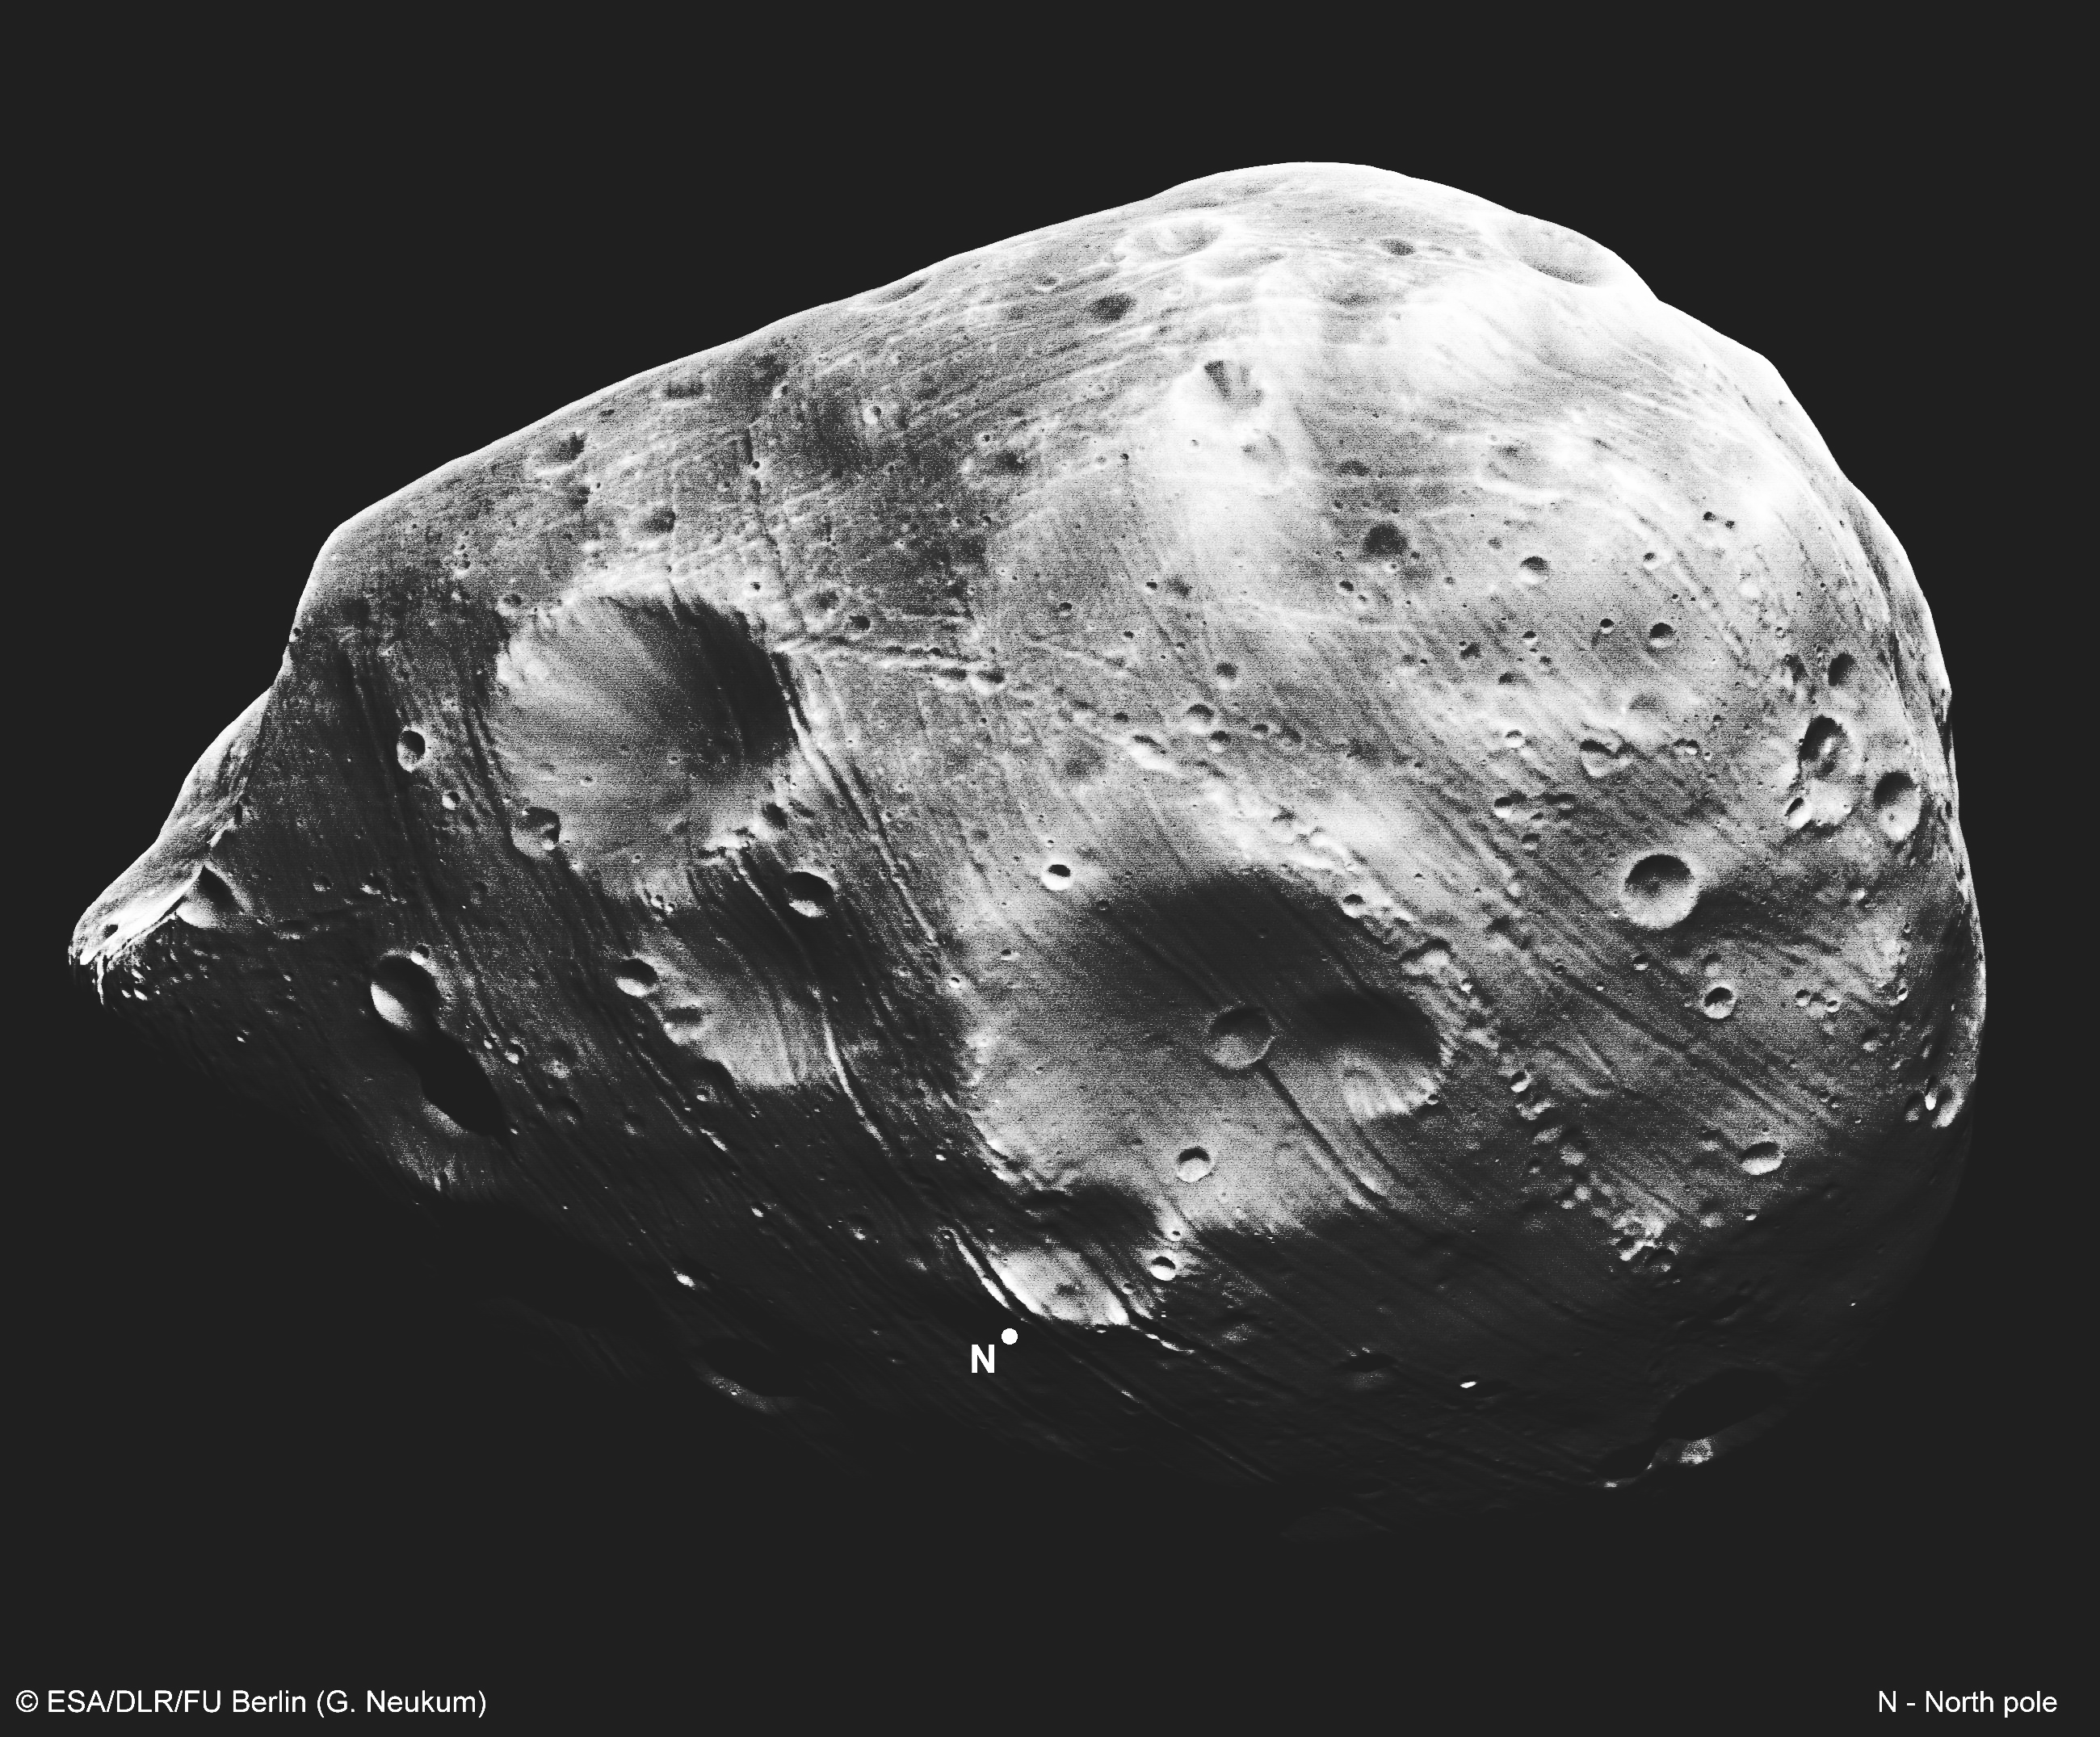
\includegraphics[width=.3\linewidth]{phobos_histmatch.png}}
 
 \subfloat[Histogram of ori\-gi\-nal ima\-ge.]{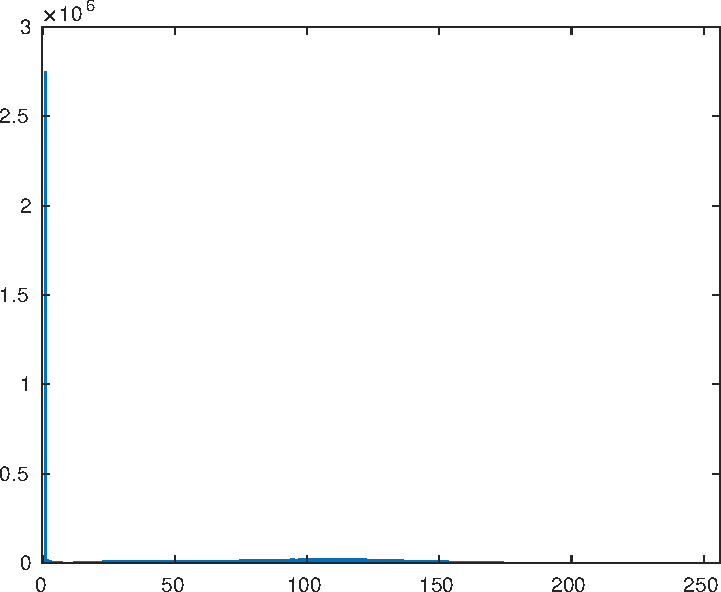
\includegraphics[width=.4\linewidth]{phobos_histogram.pdf}}\hfill
 \subfloat[Histogram after equalization.]{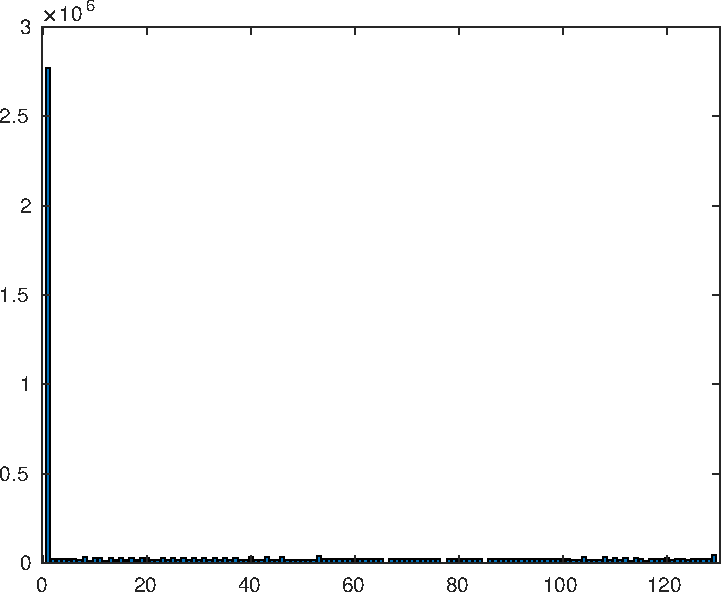
\includegraphics[width=.4\linewidth]{phobos_histogram_histeq.pdf}}
 
 \subfloat[Target histogram (probability density function).]{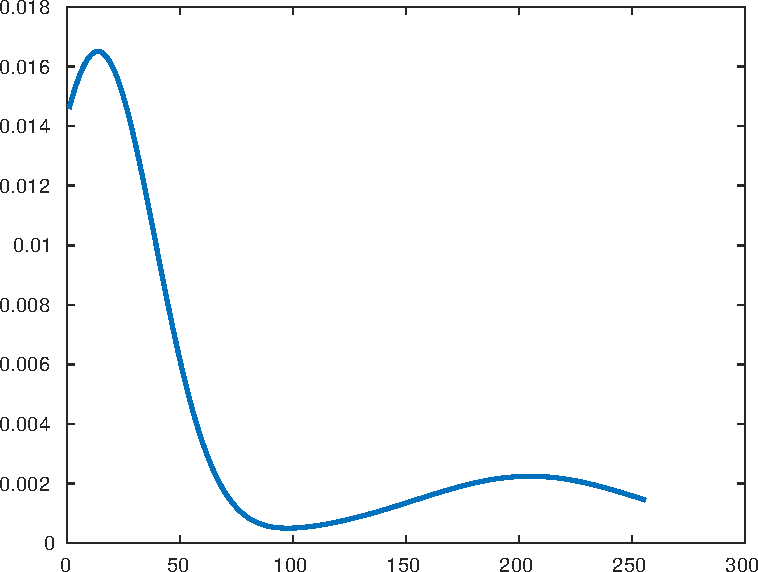
\includegraphics[width=.4\linewidth]{twomodegauss.pdf}}\hfill
 \subfloat[Histogram after histogram matching.]{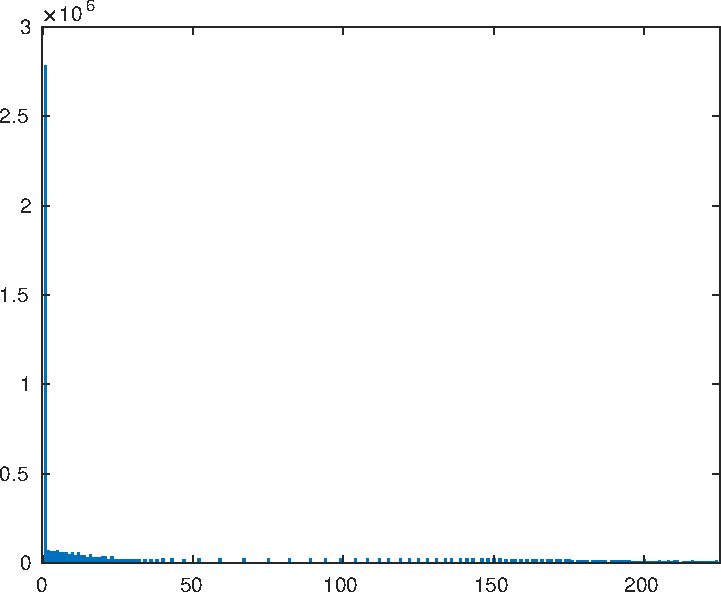
\includegraphics[width=.4\linewidth]{phobos_histogram_histmatch.pdf}}
 
 \caption{Histogram matching.}
 \label{fig:enhancement:matlab:histmatch}
\end{figure}

